\documentclass[aspectratio=169]{beamer}
% Tema utilizado. Também poderia ser:
%     Antibes       Darmstadt      Ilmenau         Marburg          Singapore
%     Bergen        Dresden        JuanLesPins     Montpellier      Szeged
%     Berkeley   [*]Frankfurt      Luebeck         PaloAlto         Warsaw 
%     Berlin        Goettingen     Madrid          Pittsburgh       boxes
%     Copenhagen    Hannover       Malmoe          Rochester        default

\mode<presentation>
{
  \usetheme{Frankfurt}
  \setbeamercovered{transparent}
}

\usepackage[portuguese]{babel}
\usepackage[utf8]{inputenc}
\usepackage{times}
\usepackage[T1]{fontenc}
\usepackage[absolute,overlay]{textpos}

\setbeamertemplate{itemize items}[ball]
\setbeamertemplate{itemize subitem}[default]
\setbeamertemplate{itemize subsubitem}{$\rightarrow$}

%*****************
% PYMPRESS OPTIONS
%*****************
%\usepackage{pgfpages}
%\setbeameroption{show notes on second screen}
%\usepackage{multimedia}

%*****************
% CITATION OPTIONS
%*****************
\usepackage[citestyle=authoryear-comp, style=authoryear-comp, uniquename=false, maxcitenames=2, maxbibnames=9]{biblatex}
\renewcommand*{\nameyeardelim}{\addcomma\addspace}
\addbibresource{./referencias.bib}
\setbeamertemplate{caption}[numbered]
\beamertemplatenavigationsymbolsempty

%****************
% CAPTION OPTIONS
%****************
\usepackage{caption}
  \setbeamerfont{caption}{series=\normalfont,size=\fontsize{8}{10}} 
  \newcommand{\source}[1]{\caption*{Fonte: {#1}} }
  \setbeamertemplate{caption}[numbered]
  \setbeamercolor{caption name}{fg=structure!0!black}
  \let\oldparencite=\parencite
  \renewcommand{\parencite}[1]{\textcolor[rgb]{0,0,.6}{\oldparencite{#1}}}


%*********************
% JUSTIFY TEXT OPTIONS
%*********************  
\usepackage{ragged2e} 
  \addtobeamertemplate{block begin}{}{\justifying}
  \addtobeamertemplate{alertblock begin}{}{\justifying}

%**************
% BLOCK OPTIONS
%**************
\newenvironment<>{blockMargin10}[1]{%
 \begin{actionenv}#2%
 \def\insertblocktitle{\leftskip=10pt\rightskip=10pt\vspace{10pt} #1\vspace{10pt}}%
 \par%
 \usebeamertemplate{block begin}\leftskip=10pt\rightskip=10pt\vspace{10pt}}
 {\par\vspace{10pt}\usebeamertemplate{block end}
 \end{actionenv}}

 \newenvironment{variableblock}[4]{%
  \setbeamercolor{block title}{#2}
  \setbeamercolor{block body}{#3}
  \setbeamercolor{item projected}{#4}
  \begin{block}{#1}}{\end{block}}

%****************
% THANKS OPTIONS
%**************** 
\makeatletter
\let\beamer@writeslidentry@miniframeson=\beamer@writeslidentry%
\def\beamer@writeslidentry@miniframesoff{%
  \expandafter\beamer@ifempty\expandafter{\beamer@framestartpage}{}% does not happen normally
  {%else
    % removed \addtocontents commands
    \clearpage\beamer@notesactions%
  }
}
\newcommand*{\miniframeson}{\let\beamer@writeslidentry=\beamer@writeslidentry@miniframeson}
\newcommand*{\miniframesoff}{\let\beamer@writeslidentry=\beamer@writeslidentry@miniframesoff}
\makeatother

%**************
% TIKZ OPTIONS
%**************
\usepackage{tikz}
\usepackage{aobs-tikz}
\tikzset{invisible/.style={opacity=0.2}}

\newcommand{\includegraphicswithwisibility}[3]{
  \begin{tikzpicture}
  \node[visible on={#1}] at (0,0) {\includegraphics[#2]{#3}};
  \end{tikzpicture}
}

\tikzstyle{decision} = [diamond, draw, fill=blue!20, 
    text width=4.5em, text badly centered, node distance=3cm, inner sep=0pt]
\tikzstyle{block} = [rectangle, draw, thick,%fill=blue!20, 
    text width=6em, text centered, rounded corners, minimum height=4em]
\tikzstyle{line} = [draw, -triangle 45]
\tikzstyle{cloud} = [draw, ellipse,fill=red!20, node distance=3cm,
    minimum height=2em]


\setbeamertemplate{footline}
{
    \leavevmode
    \hbox{
        \hspace{-2mm}
        \begin{beamercolorbox}[wd=.34\paperwidth,ht=2.5ex,dp=1.125ex,leftskip=.3cm plus1fill,rightskip=.3cm,center]{author in head/foot}
          \usebeamerfont{author in head/foot}\insertshortauthor
       \end{beamercolorbox}

      \begin{beamercolorbox}[wd=.33333\paperwidth,ht=2.5ex,dp=1.125ex,leftskip=.3cm,rightskip=.3cm plus1fil,center]{title in head/foot}
        \usebeamerfont{title in head/foot}\insertshortinstitute
      \end{beamercolorbox}

      \begin{beamercolorbox}[wd=.33333\paperwidth,ht=2.5ex,dp=1.125ex,leftskip=.3cm plus1fill,rightskip=.3cm]{author in head/foot}
        \usebeamerfont{title in head/foot}
        \insertframenumber{} / \inserttotalframenumber\hspace*{2ex}
      \end{beamercolorbox}
    }
    \vskip0pt
}
\makeatother 

\title[]{HLA e Microsserviços: Uma Aplicação para
Simulação Distribuída}

%\subtitle{Uma Exploração para Aplicabilidade em Cenários Operacionais}

\author[da Costa Neto et al]{
  Oswaldo Segundo da Costa Neto\inst{1}\\\and Carlos Magno Oliveira de Abreu\inst{2}\\\and Marcelo Alexandre Martins da Conceição\inst{1}\\\and André Benzi Baccarin\inst{1}\\\and Adilson Marques da Cunha\inst{1}
}

\institute[SIGE 2021]{
  \inst{1}%
  Instituto Tecnológico de Aeronáutica
  \and  
  \inst{2}%
  Centro de Análises de Sistemas Navais
}

\date[]{}

\subject{}

\pgfdeclareimage[height=0.6cm]{university-logo}{figs/sige.png}
\logo{\pgfuseimage{university-logo}}
\newcommand{\nologo}{\setbeamertemplate{logo}{}}

\AtBeginSection[]
{
  {
    \setbeamertemplate{footline}{} 
    \begin{frame}[noframenumbering]
      \frametitle{Roteiro}
      \tableofcontents[currentsection]
    \end{frame}
  }
}

%############################################################################
%##############################  INÍCIO  ####################################
%############################################################################

\begin{document}

%****************************************************************************
%                 CAPA
%****************************************************************************
{
\usebackgroundtemplate{
\includegraphics[width=\paperwidth]{figs/template_Slide1_apresentacoes.png}}%
\begingroup
  %\setbeamertemplate{headline}[default]
  \begin{frame}[plain]
    %\titlepage
    %\vspace{-.8cm}
    %\begin{figure}[ht!]
      %\centering
      %
\includegraphics[width=.25\linewidth]{figs/sige-capa.png}
    %\end{figure}
    %\vspace{-.3cm}
    \vspace{1.3cm}
    \begin{center}
      \usebeamerfont*{frametitle}
      \textcolor{white}{HLA e Microsserviços: Uma Aplicação para Simulação Distribuída}
    \end{center}
    \begin{textblock*}{5cm}(11.8cm,6.2cm)
      \fontsize{6.7pt}{7.2}\selectfont
      Oswaldo S. da Costa Neto - ITA\\Carlos Magno O. de Abreu - CASNAV\\Marcelo A. M. da Conceição - ITA\\André Benzi Baccarin - ITA\\Adilson Marques da Cunha - ITA
    \end{textblock*}

    \note{
      \begin{itemize}
        \item Saudação à todos que estão assistindo
        \item Vou apresentar o trabalho \textbf{TÍTULO}
        \item Realizado pelos \textbf{AUTORES}
      \end{itemize}
    }

  \end{frame}
\endgroup
}



%****************************************************************************
%                 OBJETIVO
%****************************************************************************

\begin{frame}{Objetivo}
  \begin{blockMargin10}{}
    Apresentar uma abordagem para o desenvolvimento e execução de simulações distribuídas estruturadas no \textit{framework} HLA utilizando microsserviços. 
  \end{blockMargin10}
\end{frame}

%****************************************************************************
%                 ROTEIRO
%****************************************************************************

\begin{frame}[noframenumbering]
  \frametitle{Roteiro}
  \tableofcontents
\end{frame}

%****************************************************************************
%                 INTRODUÇÃO
%****************************************************************************
\begingroup
\section{Contextualização}
\begin{frame}{Contextualização}
  \only<1>{
    \begin{figure}[ht!]
      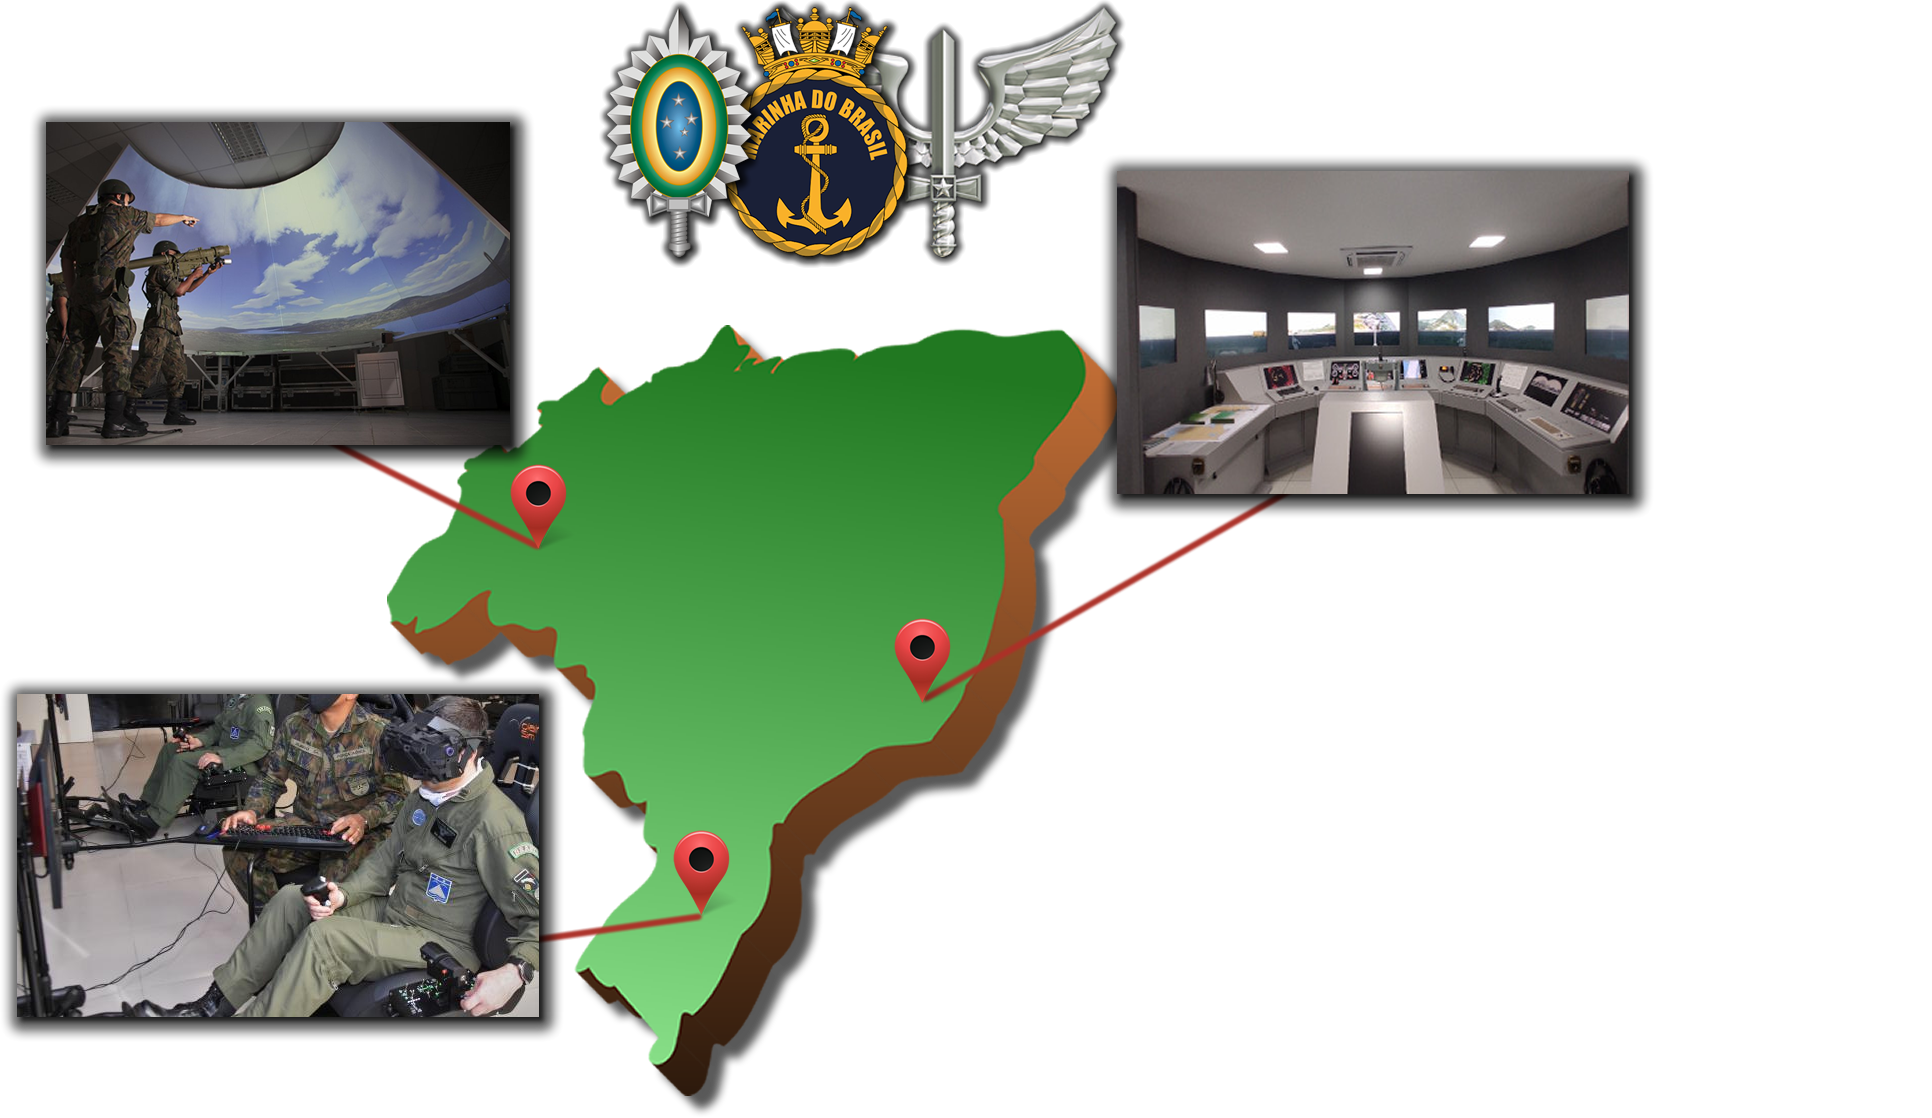
\includegraphics[width=.72\linewidth]{figs/cenario-atual1.png}
      \vspace{-0.15cm}
      \caption{\centering Forças Armadas do Brasil utilizando o conceito de Simulação como um serviço}
    \end{figure}
  }
  \only<2>{
    \begin{figure}[ht!]
      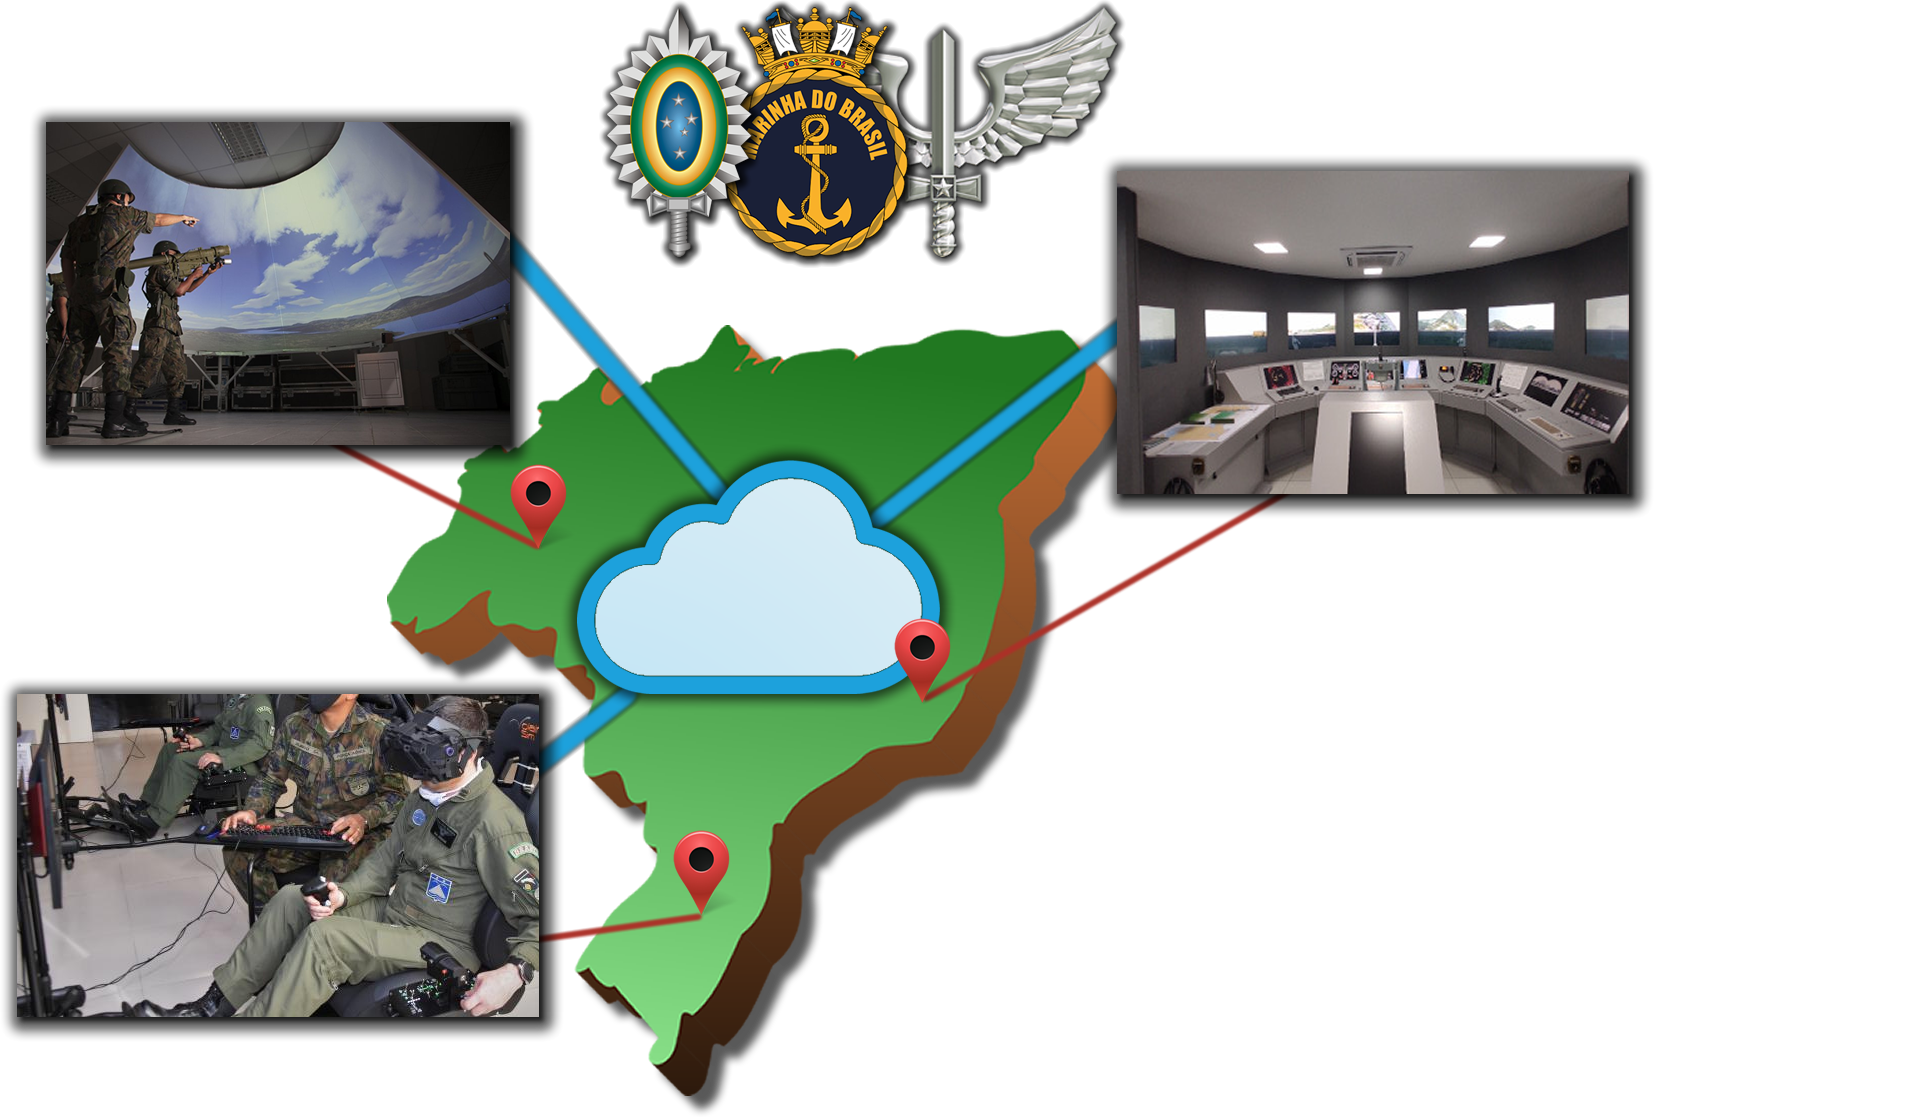
\includegraphics[width=.72\linewidth]{figs/cenario-atual2.png}
      \vspace{-0.15cm}
      \caption{\centering Forças Armadas do Brasil utilizando o conceito de Simulação como um serviço}
    \end{figure}
  }
  \only<3>{
    \begin{figure}[ht!]
      \includegraphics[width=.72\linewidth]{figs/cenario-atual3.png}
      \vspace{-0.15cm}
      \caption{\centering Forças Armadas do Brasil utilizando o conceito de Simulação como um serviço}
    \end{figure}
  }

  \note<1>{
    \begin{itemize}
      \item FAB e FFAA $\rightarrow$ diversos simuladores e sistemas \textbf{monolíticos}
      \item A interoperabilidade de dados e de sistemas é primordial para atividade de C2
      \item Importância da simulação
      \begin{itemize}
        \item Apoio à decisão
        \item Estratégia
        \item Treinamento
      \end{itemize}
    \end{itemize}
  }
  \note<2>{
    \begin{itemize}
      \item Uma solução moderna $\rightarrow$ \textit{Cloud Computing} e microsserviços
      \item Sem uma estrutura como essa ocorre:
      \begin{enumerate}
        \item Perda de capacidade de análise de Cenários Operacionais 
        \item Diminuição no potencial de treinamento 
      \end{enumerate}
    \end{itemize}
  }
  \note<3>{
    \begin{itemize}
      \item Uma abordagem moderna abre diversas possibilidades
      \begin{itemize}
        \item Conteinerização e Clusterização de sistemas
        \item Processamento paralelo
        \item Armazenamento e análise de grande conjunto de dados
        \item E o foco deste trabalho, \textbf{SIMULAÇÃO DISTRIBUÍDA}
      \end{itemize}
    \end{itemize}
  }
\end{frame}

%\begin{frame}{A Evolução das Arquiteturas de Simulação Distribuída}
%  \begin{figure}[ht!]
%    \centering
%    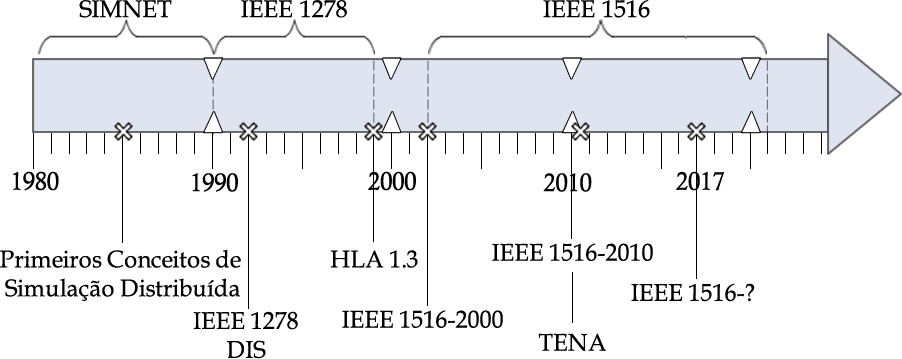
\includegraphics[width=.65\linewidth]{figs/timeline.png}
%    \caption{\centering Evolução das arquiteturas de Simulação Distribuída}
%    \vspace{-0.5cm}
%    \source{Adaptado de \parencite{Okan2017}}
%  \end{figure}
%  \note{
%    \begin{itemize}
%      \item Década de 1980 $\rightarrow$ início dos estudos com o  Projeto %\textit{SIMulation NETworking} pelo DoD com objetivo de %intercomunicar seus sistemas computacionais de simulação.
%      \item Evolução do SIMNET $\rightarrow$ Criação de padrões %industriais como o  \textit{Distributed Interactive Simulation} (DIS)%.
%      \item Meados dos anos 2000 $\rightarrow$ Esforços contínuos %liderados pelo DoD produziram um \textit{framework} para trazer uma %facilitação na interoperabilidade entre os sistemas simulados, o %\textit{High Level Architecture} (HLA).
%      \item Atualmente existem vários padrões de arquitetura de simulação %distribuída
%    \end{itemize}
%  }
%\end{frame}

\begin{frame}{Tendências de Padrões de Arquitetura}
  \hspace{-1cm}
  \begin{figure}[ht!]
    \centering
    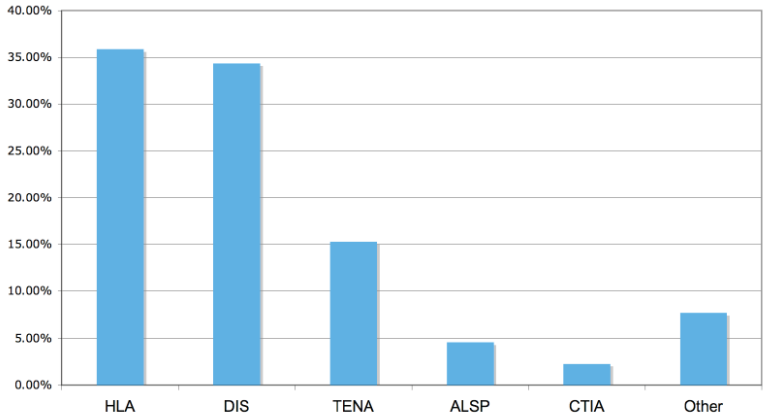
\includegraphics[width=.65\linewidth]{figs/trending-simulation-architecture.png}
    \caption{\centering Tendências de uso de arquiteturas de Simulação Distribuída}
    \vspace{-0.5cm}
    \source{\parencite{Salio2012}}
  \end{figure}

  \note{
    \begin{itemize}
      \item Os padrões mais utilizados na atualidade
      \item Destaque para HLA e DIS
    \end{itemize}
  }
\end{frame}

\begin{frame}{Topologias de Simulações Distribuídas}
  \centering
  \begin{columns}
    \begin{column}{.5\textwidth}
      \centering \textbf{DIS}
      \begin{figure}[ht!]
        \centering
        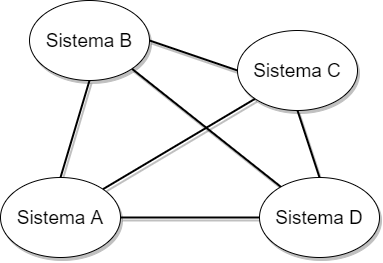
\includegraphics[width=.58\linewidth]{figs/Topology-parwise.png}
        \caption{\centering Topologia do tipo \textit{pair-wise integration}}
      \end{figure}
    \end{column}
    \begin{column}{.5\textwidth}
      \centering \textbf{HLA}
      \begin{figure}[ht!]
        \centering
        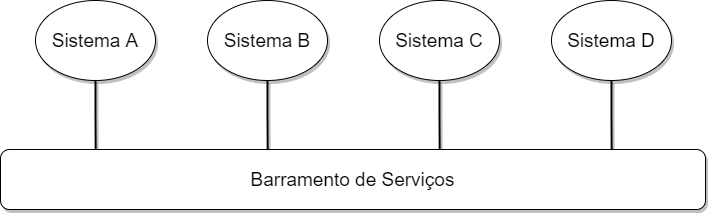
\includegraphics[width=1\linewidth]{figs/Topology-service-bus.png}
        \caption{\centering Topologia do tipo \textit{bus-service}}
      \end{figure}
    \end{column}
  \end{columns}

  \note{
    \begin{itemize}
      \item \textbf{DIS}: 
      \begin{enumerate}
        \item Tem uma topologia de comunicação direta entre os componentes. 
        \item É entendido como um protocolo de comunicação.
        \item PDU
        \item P2P
      \end{enumerate}
      \item \textbf{HLA}: 
      \begin{enumerate}
        \item Utiliza um barramento de comunicação.
        \item Proporciona melhor utilização do conceito de serviços. 
        \item \textit{Publish} / \textit{Subscribe}
        \item SOA
      \end{enumerate}
    \end{itemize}
  }
\end{frame}

%****************************************************************************
%                 CONCEITUALIZAÇÕES
%****************************************************************************
\section{Conceitualizações}

\begin{frame}{\textit{High Level Architecture} (HLA)}
  \vspace{-0.4cm}
  \only<1>{
    \begin{figure}[ht!]
      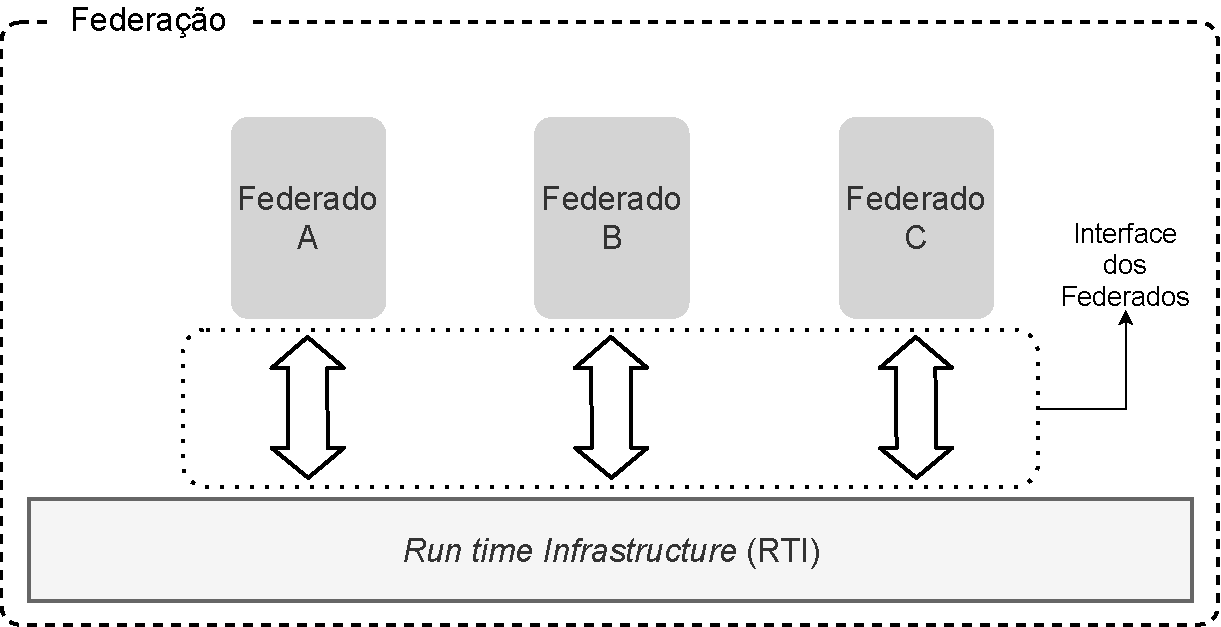
\includegraphics[width=.6\linewidth]{figs/rti.pdf}
      \vspace{-0.15cm}
      \caption{\centering Componentes de um cenário operacional a partir de uma Federação HLA}
    \end{figure}
  }
  \only<2>{
    \begin{figure}[ht!]
      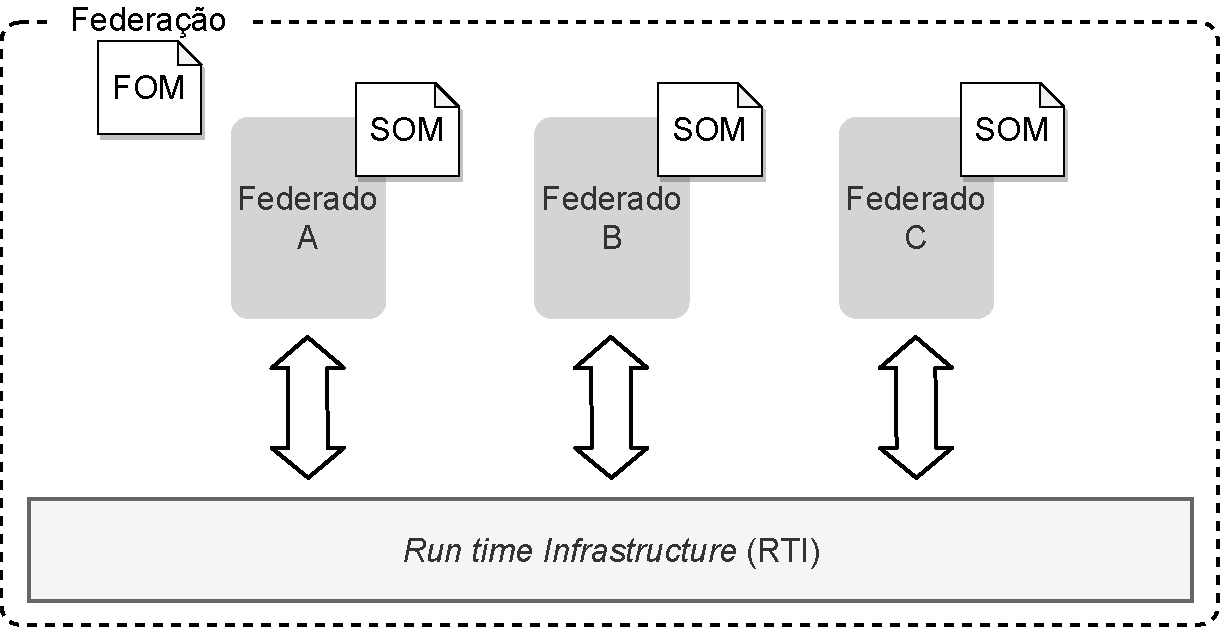
\includegraphics[width=.6\linewidth]{figs/rti-fom.pdf}
      \vspace{-0.15cm}
      \caption{\centering Componentes de um cenário operacional a partir de uma Federação HLA}
    \end{figure}
  }

  \note<1>{
    \begin{itemize}
      \item \textit{Framework} estruturado em um conjunto de regras (10) para interação dos componentes de uma forma determinada no contexto da simulação.
      \item Componentes
      \begin{itemize}
        \item Federados $\rightarrow$ Unidade básica da federação, um módulo ou sistema simulado (simulador de voo; \textit{data loggers}; visualizadores 3d; etc)
        \item Interfaces $\rightarrow$ A forma como esses federados se comunicam
        \item RTI $\rightarrow$ conjunto de bibliotecas, binários como um software que os federados utilizam para se comunicar
        \item Federação $\rightarrow$ é o contexto da simulação distribuída, ou um cenário operacional 
      \end{itemize}
    \end{itemize}
  }
  \note<2>{
    \begin{itemize}
      \item Necessita de padronização dos dados dos sistemas
      \item \textit{Templates} HLA $\rightarrow$ SOM e FOM
      \item SOM $\rightarrow$ Declaração \textit{publish}/\textit{subscribe} (como em serviços de mensageria)
      \item FOM $\rightarrow$ Comum a todos os federados
      \item SOM é obtido a paritr de um FOM
    \end{itemize}
  }
\end{frame}

\begin{frame}{\textit{High Level Architecture} (HLA)}
  \vspace{-3cm}
  \vfill\null
  \begin{columns}
    \begin{column}{.5\textwidth}
      \begin{figure}[ht!]
        \centering
        \includegraphicswithwisibility{<1>}{width=1\linewidth}{figs/crc.png}
        \uncover<1>{\caption{\centering Representação de uma RTI centralizada}}
      \end{figure}
    \end{column}
    \begin{column}{.5\textwidth}
      \begin{figure}[ht!]
        \centering
        \includegraphicswithwisibility{<2>}{width=.65\linewidth}{figs/lrc.png}
        \uncover<2>{\caption{\centering Representação de uma RTI descentralizada}}
      \end{figure}
    \end{column}
  \end{columns}
  
  \note<1>{
    \begin{itemize}
      \item Quanto ao gerenciamento dos processos relativos à uma execução de simulação
      \item RTI pode ser centralizada, com a presença de um CRC
      \item Realiza o controle dos eventos principais e regulagem temporal 
    \end{itemize}
  }
  \note<2>{
    \begin{itemize}
      \item Ou descentralizada, sem a presença de um CRC
      \item Nesse caso, todos os federados são igualmente responsáveis pelo gerenciamento e manutenção dos eventos da simulação
      \item \textbf{ESSA ABORDAGEM TEM MAIS CORRELAÇÃO COM OS CONCEITOS DE MICROSSERVIÇOS}
      \begin{itemize}
        \item Modularização
        \item baixo acoplamento
        \item reutilização
        \item etc
      \end{itemize}
    \end{itemize}
  }
\end{frame}



\begin{frame}{Microserviços: Máquinas Virtuais X Docker}
  \vspace{-3cm}
  \vfill\null
  \begin{columns}
    \begin{column}{.5\textwidth}
      \begin{figure}[ht!]
        \centering
        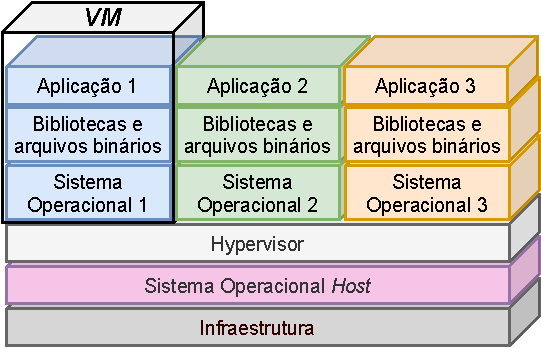
\includegraphics[width=.8\linewidth]{figs/estrutura-vm.pdf}
        \vspace{-.15cm}
        \caption{\centering Virtualização clássica com VMs}
      \end{figure}
    \end{column}
    \begin{column}{.5\textwidth}
      \begin{figure}[ht!]
        \centering
        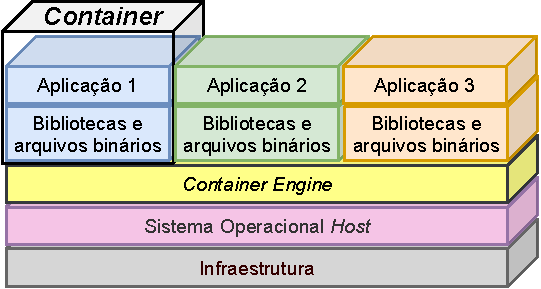
\includegraphics[width=.8\linewidth]{figs/estrutura-container.pdf}
        \vspace{-.15cm}
        \caption{\centering Virtualização \textit{lightweight} com \textit{containers}}
      \end{figure}
    \end{column}
  \end{columns}
  
  \note{
    \begin{itemize}
      \item Duas formas principais de se obter virtualização com microsserviços:
      \begin{itemize}
        \item Máquinas Virtuais
        \item \textit{Containers} $\rightarrow$ baseado em containers Linux
      \end{itemize}
      \item Ambas abordagens tem vantagens e desvantagens, mas os pontos em comum são
      \begin{itemize}
        \item isolamento de sistemas
        \item modularização 
        \item baixo acoplamento
        \item reusabilidade, entre outros
      \end{itemize} 
      \item Vantagem dos \textit{containers}
      \begin{itemize}
        \item Abstração da camada de hardware 
        \item Virtualização das chamadas do sistema operacional (não é baseado em \textit{hypevisor})
        \item Aplicações mais leves que utilizam menos recursos (mais eficientes)
      \end{itemize}
    \end{itemize}
  }
\end{frame}

\begin{frame}{Microserviços com Docker \textit{Containers}}

  \begin{columns}
    \begin{column}{.5\textwidth}
      \begin{blockMargin10}{}
        \begin{itemize}
          \item Conteinerização de Federados HLA
          \item Orquestração e Coreografia
          \item Simulação como um serviço
          \item Interoperabilidade de Sistemas
        \end{itemize}
      \end{blockMargin10}
    \end{column}
    \begin{column}{.5\textwidth}
      \vspace{-1cm}
      \vfill\null
      \begin{figure}[ht!]
        \centering
        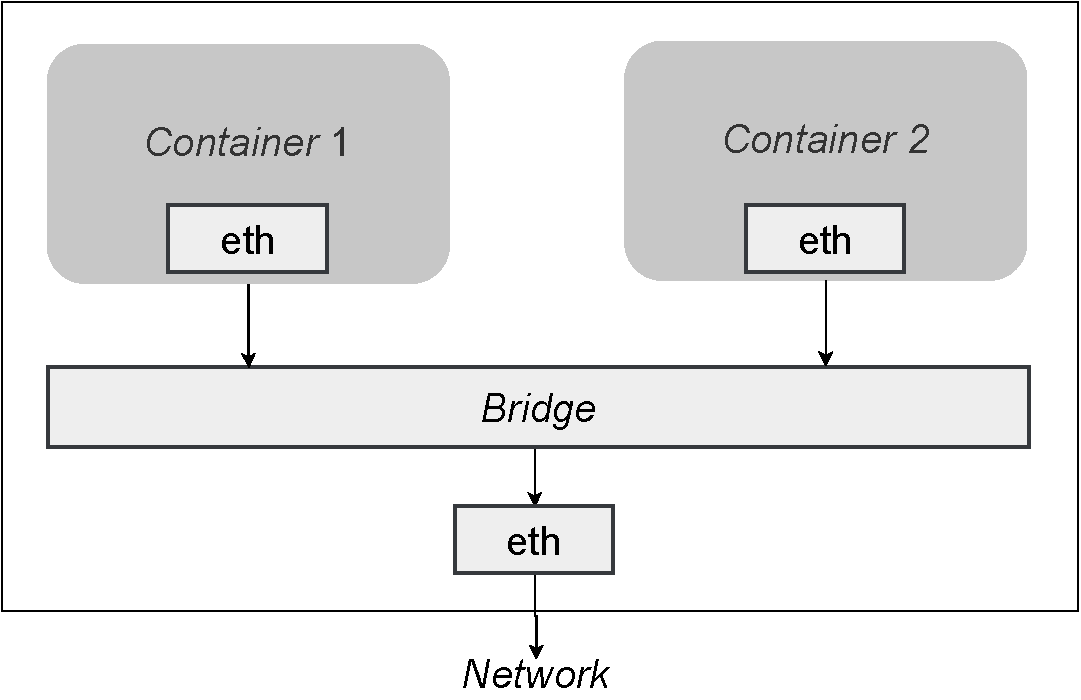
\includegraphics[width=.75\linewidth]{figs/bridge.pdf}
        \vspace{-.15cm}
        \caption{\centering Rede Docker em Formato \textit{Bridge}}
      \end{figure}
    \end{column}
  \end{columns}
  
  \note{
    \begin{itemize}
      \item Docker é a ferramenta mais comum de obtenção de microsserviços com base em \textit{containers}
      \item Perceba que a topologia é análoga ao HLA
      \item \textcolor{blue}{Cada container é equivalente a um Federado, ou seja, a CONTEINERIZAÇÃO DOS FEDERADOS}
      \item A rede RTI pode transitar na placa de rede padrão Docker (bridge) ou externamente com camadas de sobreposição de rede \textit{overlay}
      \item Orquestração e Coreografia $\rightarrow$ Facilitação do desenvolvimento e manutenção com estratégias de 
      \item Coreografia dá maies evidência aos princípios de microsserviços, porque traz a ideia de descentralização de responsabilidades, promovendo o baixo acoplamento
      \item A interoperabilidade dos sistemas $\rightarrow$ O grande objetivo de uma simulação distribuída 
    \end{itemize}
  }
\end{frame}

%****************************************************************************
%                 ESTUDOS CORRELATOS
%****************************************************************************
\section{Estudos Correlatos}
\begin{frame}{Estudos Correlatos}
  \only<1>{
    \begin{figure}[ht!]
      \centering
      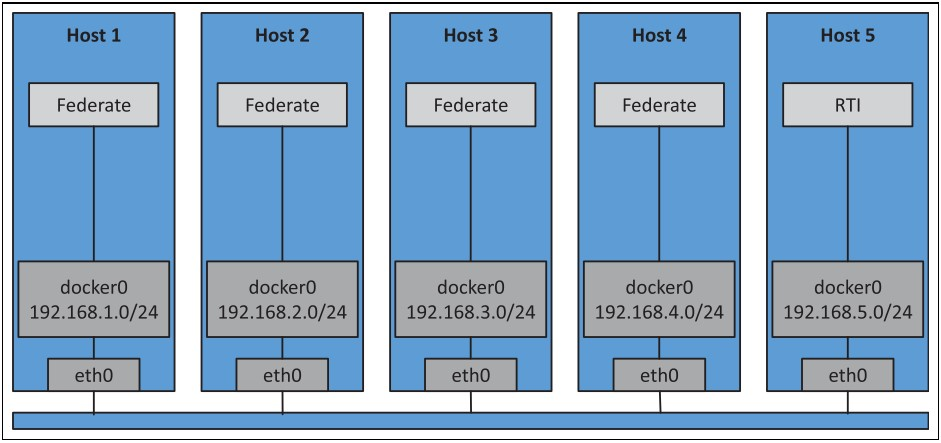
\includegraphics[width=.65\linewidth]{figs/rtiref.jpg}
      \caption{\centering Estrutura de Rede Aplicada em \parencite{VandenBerg2017}}
    \end{figure}
  }
  \only<2>{
    \begin{figure}[ht!]
      \centering
      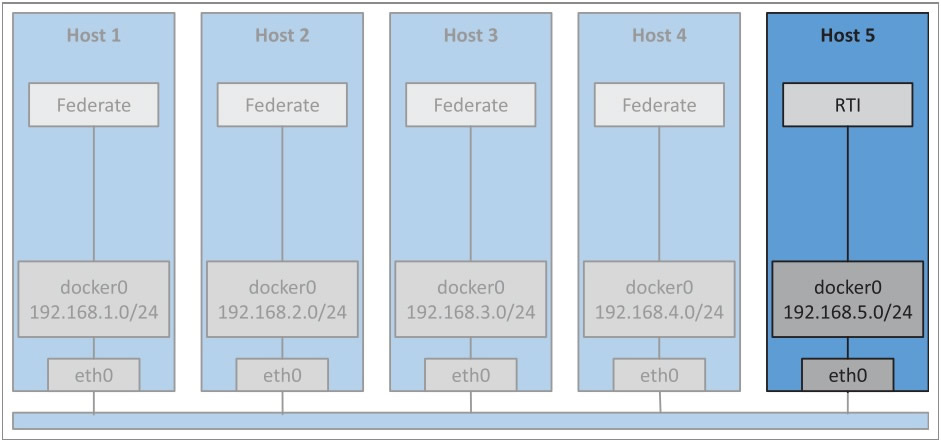
\includegraphics[width=.65\linewidth]{figs/rtiref2.jpg}
      \caption{\centering Estrutura de Rede Aplicada em \parencite{VandenBerg2017}}
    \end{figure}
  }

  \note<1>{
    \begin{itemize}
      \item Durante a pesquisa para a realização deste trabalho, foram encontradas alguns artigos que traziam abordagens similares, porém o principal correlato foi o trabalho de Van den Berg de 2017.
      \item Ele descreve modelos para obtenção de uma simulação distribuída estruturada no \textit{framework} HLA, nas ferramentas do ecossistema Docker e utilizando a RTI da Pitch.
      \item Além disso, ele faz uma série de testes para avaliar as possibilidades de uma composição HLA com diversas configurações: multiplos hosts, host único, WAN (rede de longa distancia), LAN(Rede local).  
    \end{itemize}
  }
  \note<2>{
    \begin{itemize}
      \item Porém em todos seus testes, ele elenca um \textit{container} específico para ser o gerenciador da RTI, diferente do proposto neste artigo.
      \item Existem alguns aspectos relacionados à perda de desempenho devido à latência por conta da obrigatoriedade da utilização de protocolo TCP/IP entre outros motivos que degradam a rede.
      \item A abordagem proposta que será vista traz o uso de uma RTI descentralizada com o objetivo de gerar um melhor desempenho.
    \end{itemize}
  } 

\end{frame}

%****************************************************************************
%                    ABORDAGEM PROPOSTA
%****************************************************************************
\section{Abordagem Proposta}
\begin{frame}{Abordagem Proposta}
  \vspace{-1cm}
  \begin{figure}[ht!]
    \centering
    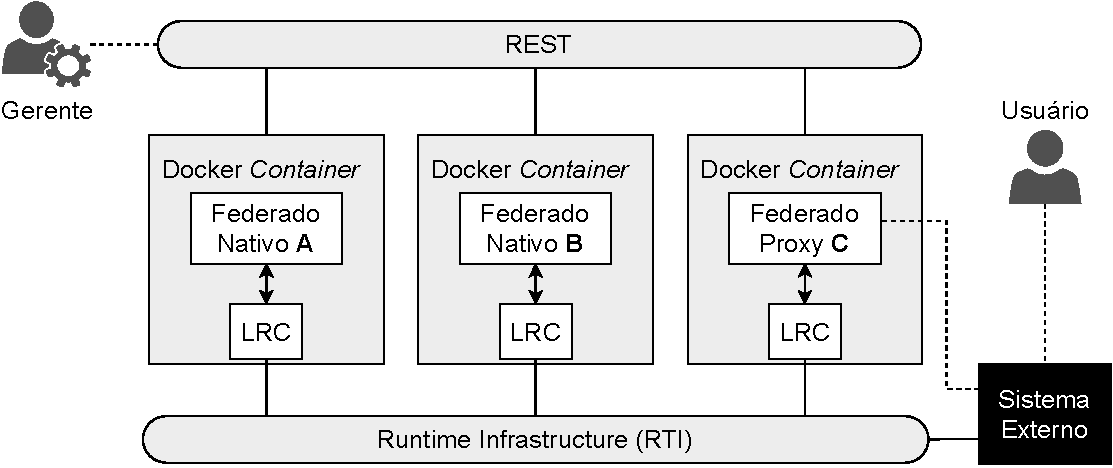
\includegraphics[width=.65\linewidth]{figs/abordagem-proposta.pdf}
    \caption{\centering Abordagem proposta para interoperabilidade de dados utilizando microsserviços}
  \end{figure}

  \note{
    \begin{itemize}
      \item Características
      \begin{itemize}
        \item Federados conteinerizados
        \item RTI descentralizada
        \item Comunicação em protocolo multicast
        \item Dupla camada de comunicação (RTI e REST)
        \item Federados podem ser
        \begin{itemize}
          \item \textbf{NATIVO:} Toda a regra de negócios do federado está internamente ao \textit{container}. 
          \item \textbf{PROXY:} Federado que obtém dados de um sistema externo (caixa-preta)
        \end{itemize}
        \item Gerente controla a execução da simulação por meio de comandos REST 
      \end{itemize}
    \end{itemize}
  }

\end{frame}

%****************************************************************************
%                    PROJETO ARCANJO
%****************************************************************************
\begin{frame}{Projeto Arcanjo}
  \begin{columns}
    \begin{column}{.2\textwidth}
      \vspace{-1cm}
      \begin{figure}[ht!]
        \centering
        
\includegraphics[width=1\linewidth]{figs/arcanjo.png}
      \end{figure}
    \end{column}
    \begin{column}{.8\textwidth}
      \vspace{-1cm}
      \begin{blockMargin10}{}
        \begin{itemize}
          \item Plataforma de Simulação Padrão OTAN
          \item Integração Entre Simuladores das Forças Armadas
          \item RPR-FOM v2.0
          \item Portico RTI
        \end{itemize}
      \end{blockMargin10}
    \end{column}
  \end{columns}

  \note{
    \begin{itemize}
      \item Para concretizar os conceitos da abordagem proposta, o estudo de caso foi feito utilizando a Plataforma do Projeto Arcanjo
      \item Desenvolvido com base nos padrões OTAN
      \item Objetivo era a integração entre simuladores das FFAA
      \item Padronização de dados com o RPR-FOM v2.0 $\rightarrow$ É o padrão OTAN utilizado para mapeamento de objetos e atributos de entidades militares 
      \item Docker Containers $\rightarrow$ o que justifica a sua escolha para a aplicação d abordagem proposta
      \item Spring Boot $\rightarrow$ \textit{framework} de código aberto para a plataforma Java utilizado para acelerar o desenvolvimento de microsserviços 
      \item Cesium $\rightarrow$ biblioteca \textit{open source} para manipulação de mapas 3D. Importante para a criação de um Federado específico para Visualização do cenário operacional
      \item \textit{Portico} $\rightarrow$ infraestrutura de código aberto para implementação de arquiteturas HLA com RTI descentralizada 
    \end{itemize}
  }

\end{frame}

%****************************************************************************
%                    ESTUDO DE CASO
%****************************************************************************
\begin{frame}{Estudo de Caso}
  \begin{columns}
    \begin{column}{.45\textwidth}
      \vspace{-.8cm}
      \begin{figure}
      \includegraphicswithwisibility{<1>}{width = .8\textheight}{figs/arcanjogeral.jpg}
      \uncover<1>{\caption{\centering Execução da simulação distribuída utilizando a abordagem proposta}}
      \end{figure}
    \end{column}
    \begin{column}{.55\textwidth}
      \vspace{-.8cm}
      \begin{figure}
      \includegraphicswithwisibility{<2>}{width = .9\textheight}{figs/map-objects.png}
      \uncover<2>{\caption{\centering Processo de Mapeamento de Objetos para RTI}}
      \end{figure}
    \end{column}
  \end{columns}

  \note<1>{
    \begin{itemize}
      \item Essa é a configuração do Estudo de caso
      \item 3 Federados. 1 nativo e 2 proxys para conectar sistemas externos
      \begin{itemize}
        \item Federado Visualizador de Mapas: Nativo e criado para visualização do cenário operacional
        \item FlightRadar: Federado Proxy criado para obter por meio de \textit{web services} o posicionamento das aeronaves reais disponível no site do FlightRadar24
        \item Xplane: Federado Proxy que capta as informações das aeronaves do simulador xplane e envia para ele as demais aeronaves que estão circulando na RTI, vindo do flightradar 
      \end{itemize}
    \end{itemize}
  }

  \note<2>{
    \begin{itemize}
      \item Mostra como é feito o mapeamento dos dados desses sistemas externos para dentro da RTI
    \end{itemize}
  }

\end{frame}

\begin{frame}{Estudo de Caso}
  \begin{columns}
    \begin{column}{.5\textwidth}
      \vspace{-.5cm}
      \begin{figure}
      \includegraphicswithwisibility{<1>}{width =1\textwidth}{figs/arcanjo-estudo-de-caso.png}
      \uncover<1>{\caption{\centering Visualização do cenário operacional por meio do Federado Visualizador de Mapas}}
      \end{figure}
    \end{column}
    \begin{column}{.5\textwidth}
      \vspace{-.5cm}
      \begin{figure}
      \includegraphicswithwisibility{<2>}{width =1\textwidth}{figs/xplane-screenshot.png}
      \uncover<2>{\caption{\centering Visão de um objeto oriundo da RTI no sistema externo X-Plane 11}}
      \end{figure}
    \end{column}
  \end{columns}

  \note{
    \begin{itemize}
      \item A utilização do 3º federado para visualizar os objetos trafegados no interior da RTI.
      \item Sistema externo xplane recebendo as informações da RTI e mostrando no simulador um objeto de aeronave de oriundo do flightradar
    \end{itemize}
  }

\end{frame}

%****************************************************************************
%                       DESEMPENHO
%****************************************************************************

\begin{frame}{Análise dos Resultados}

  \begin{columns}
    \begin{column}{.5\textwidth}
      \begin{exampleblock}<1>{\centering Vantagens}
        \begin{itemize}
          \item Modularização de sistemas
          \item Descentralização
          \item Velocidade no desenvolvimento
          \item Reusabilidade
          \item Escalabilidade
        \end{itemize}
      \end{exampleblock}
    \end{column}
    \begin{column}{.5\textwidth}
      \begin{alertblock}<2>{\centering Desvantagens}
        \begin{itemize}
          \item Comunicação $\rightarrow$ Camada 3 do modelo OSI
          \item IP Multicast
          \begin{itemize}
            \item RTI descentralizada
            \item Docker
          \end{itemize} 
        \end{itemize}
      \end{alertblock}
    \end{column}
  \end{columns}

  \note<1>{
    \begin{itemize}
      \item Todos os pontos de vantagens são interligados com as próprias capacidades de microsserviços
      \item Destaque para a Escalabilidade, que é obtida quando se utiliza computação em nuvem e microsserviços como kubernetes e a clusterização dos containers, abrindo maiores possibilidades pra obter um maior poder computacional na solução de problemas de simulação 
    \end{itemize}
  }
  \note<2>{
    \begin{itemize}
      \item Perda de desempenho devido ao acréscimo de camadas na cominicação entre as aplicações.
      \item Estudos $\rightarrow$ perda de desempenho causada pela virtualização em torno de 3,33\% em relação aos mesmos aplicativos estruturados de forma monolitica em máquinas físicas. 
      \item Apesar da vantagem do protocolo Multicast na eficiência do uso da largura de banda, ele requer uma configuração especial da infraestrutura de rede ou o uso de ferramentas de roteamento baseadas em software.
      \item O Docker não aceita a criação de uma camada de sobreposição de rede para múltiplos \textit{hosts} em configuração multicast. Para isso é necessário uso de ferramentas como o Weave Router.
    \end{itemize}
  }

\end{frame}

\renewcommand{\parencite}[1]{\textcolor[rgb]{1,1,1}{\oldparencite{#1}}}
\begin{frame}{Desempenho}
  \begin{figure}[ht!]
    \hspace{-1cm}
    \centering
    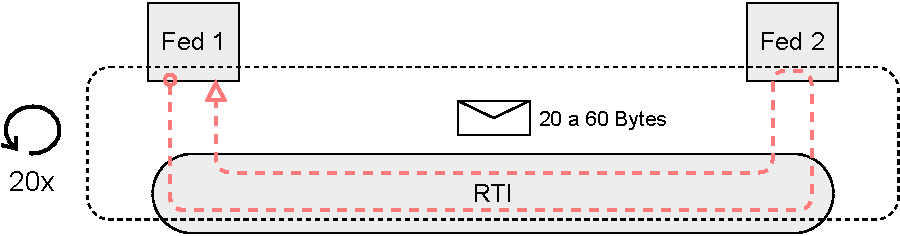
\includegraphics[width=.8\linewidth]{figs/test-latency.pdf}
    \caption{\centering Esquema do teste de latência entre os Federados}
  \end{figure}

  \begin{columns}
    \begin{column}{.225\textwidth}\end{column}
    \begin{column}{.275\textwidth}
      \begin{block}{\centering \parencite{VandenBerg2017}}
        \vspace{.1cm}
        \centering
        $\downarrow$ 16 - 26\%
        \vspace{.1cm}
      \end{block}
    \end{column}
    \begin{column}{.275\textwidth}
      \begin{block}{\centering Abordagem proposta}
        \vspace{.1cm}
        \centering
        $\downarrow$ 7.6\%
        \vspace{.1cm}
      \end{block}
    \end{column}
    \begin{column}{.225\textwidth}\end{column}
  \end{columns}

  \note{
    \begin{itemize}
      \item Para verificar o desempenho da abordagem proposta, foi realizado um teste de performance.
      \item Os parâmetros de execução do teste foram extraídos do trabalho de van den berg para haver uma comparação dos Resultados
      \item Teste
      \begin{itemize}
        \item Dois Federados com função exclusiva de trocar pacotes de dados de 20 a 60 bytes
        \item Pacote sai do FED 1 viaja pela RTI é recebido e reenviado pelo FED 2, viaja novamente e retorna ao FED 1
        \item repetição desses passos 20x
      \end{itemize}
      \item Vandenberg obteve 16 a 26\% de perda de desempenho quando comparado com uma RTI nativa, sem uso de \textit{containers}
      \item A nossa abordagem proposta teve perda de 7.6\% comparado com a mesma referência, uma RTI nativa sem o uso de containers.
      \item Diferença de resultados está atrelada à configuração multihost
    \end{itemize}
  }

\end{frame}

%****************************************************************************
%                 Conclusão
%****************************************************************************
\section{Conclusão}

\begin{frame}{Conclusão}

  \begin{blockMargin10}{}
    \begin{itemize}
      \item<1> Simulação Distribuída e Microsserviços $\rightarrow$ \textit{Cloud Computing}
      \vspace{.1cm}
      \item<2> Prova de conceito $\rightarrow$ Modularização de aplicações monolíticas
      \vspace{.1cm}
      \item<3> RTI descentralizada $\rightarrow$ Redução da complexidade arquitetural
      \vspace{.1cm}
      \item<4> Desempenho $\rightarrow$ Simulações baseadas em tempo real
    \end{itemize}
  \end{blockMargin10}

  \note{
    \begin{itemize}
      \item Utilizar microsserviços para obter simulações distribuídas é uma forte tendência na comunidade de modelagem e simulação, principalmente atrelada ao paradigma de computação em nuvem
      \item A prova de conceito mostrou a possibilidade da modularização das aplicações de simulação com o objetivo de interoperar dados
      \item A escolha por uma RTI descentralizada traz diversos benefícios, incluindo uma considerável redução da complexidade de desenvolvimento dos Federados
      \item O desempenho em métricas como a latência é essencial para a obtenção de simulações baseadas em tempo real, como por exemplo em simuladores de voo.
    \end{itemize}
  }

\end{frame}
\endgroup

%****************************************************************************
%                 ROTEIRO
%****************************************************************************

\begin{frame}[noframenumbering]
  \frametitle{Roteiro}
  \tableofcontents
\end{frame}

%****************************************************************************
%                 OBJETIVO
%****************************************************************************
\miniframesoff  
\begin{frame}[noframenumbering]{Objetivo}
  \begin{blockMargin10}{}
    Apresentar uma abordagem para o desenvolvimento e execução de simulações distribuídas estruturadas no \textit{framework} HLA utilizando microsserviços. 
  \end{blockMargin10}
\end{frame}

%****************************************************************************
%                       BIBLIOGRAFIA
%****************************************************************************

%\appendix
%\setbeamercolor{bibliography entry author}{fg=blue}
%\setbeamercolor{bibliography entry title}{fg=black} 
%\setbeamercolor{bibliography entry location}{fg=blue} 
%\section{Apêndice}   
%\begin{frame}[t, allowframebreaks]{Referências}
%  \printbibliography
%\end{frame} 

%****************************************************************************
%                              CONTATOS
%****************************************************************************
\miniframesoff  
\begingroup
  \AtBeginSection[]{}
  \section{} 
  \begin{frame}[noframenumbering, plain]{}
    \centering
    \vspace{.8cm}
    {\Large
    Obrigado!}
    \vspace{.5cm}
    \begin{columns}
      \begin{column}{.25\textwidth}\end{column}
      \begin{column}{.5\textwidth}
        \begin{block}{\centering Contatos}
          \centering
          oswaldocostaneto@hotmail.com\\
          magno.mabreu@gmail.com\\
          marcelomamc88@gmail.com\\
          baccarin.andre@gmail.com\\
          cunha.adilsonmarques@gmail.com
        \end{block}
      \end{column}
      \begin{column}{.25\textwidth}\end{column}
    \end{columns}
    \vspace{.5cm}
    \begin{figure}[ht!]
      \centering
      
\includegraphics[width=.4\linewidth]{figs/sige-capa.png}
    \end{figure}
  \end{frame} 
\endgroup


\end{document}



